\documentclass[a4paper,11pt]{article}
\usepackage[utf8]{inputenc}
\usepackage[T1]{fontenc}
\usepackage[french]{babel}
\usepackage[right=2.5cm, left=2.5cm, bottom=4cm, top=3cm]{geometry}
\usepackage{textcomp}
\usepackage{graphicx}
\usepackage{mathtools,amssymb,amsthm}
\usepackage{lmodern}
\usepackage{multirow}
\usepackage{array}
\usepackage{longtable}

\title{\vspace{13em}{\huge Cahier des Charges}}
\author{Edouard Fouassier - Maxime Gonthier - Benjamin Guillot\\
		Laureline Martin - Rémi Navarro - Lydia Rodrigez de la Nava
		\vspace{2em}\\
		Algorithme Genetique
		\vspace{2em}}

\begin{document}
	
	\pagenumbering{gobble}\clearpage
	\maketitle\vspace{13em}
\newpage
\tableofcontents
\newpage\clearpage\pagenumbering{arabic}
	
	\section*{Introduction}
		Le nom algorithme génétique vient des ressemblances avec le monde du vivant, il y a en effet des mutations, des générations et de la sélection naturelles pour n’en citer que quelques uns. 
		Cet algorithme a été étudié par John Holland de 1960 à 1975 dans son ouvrage Adaptation in Natural and Artificial System inspiré entre autres par la “learning machine” de Turing.\\
		\\
		L’algorithme génétique s’applique à une grande variété de domaines. 
		Tout d’abord, il peut s’appliquer en génétique pour étudier l’évolution des gènes d’une espèce donnée sur plusieurs générations. 
		On peut aussi appliquer l’algorithme dans le cas d’apprentissage comme par exemple apprendre à un robot à se déplacer en fonction des obstacles. 
		Un troisième domaine d’application possible est l’optimisation. 
		On peut citer dans cette catégorie l’optimisation de portefeuille d'action en fonction de leurs risques ou bien l’optimisation de la ventilation dans le cas de feu dans des espaces confinées ou bien simplement l’optimisation d’une fonction.\\ 
		\\
		L’algorithme génétique est particulièrement utile lorsque l’utilisateur étudie une population et qu’il recherche une solution approchée parmi ces valeurs. 
		Les algorithmes génétiques se démarquent des autres car ils sont très facilement adaptables à différents problèmes. 
		On utilise des règles de transition probabiliste, ce qui est pertinent pour des problèmes où les résultats sont des valeurs approchées.\\

	\section{Fondement du projet}
		\subsection{But du projet}
			L'objectif du projet est de réaliser un programme utilisant un algorithme génétique permettant de délivrer une solution ou un ensemble de solutions optimale(s) d’un problème donné à l’utilisateur en fichier de sortie.
		
		\subsection{Personnes et organismes impliqués dans les enjeux du projet}
			Le projet a pour client principal madame Leila Kloul.
			
		\subsection{ Utilisateurs du produit}
			Le produit se veut se veut employable par n’importe qui cherchant une réponse adaptée à un problème d’optimisation lié à une fonction.
			
	\section{Contraintes sur le projet}
		\subsection{Contraintes non négociables}
			Le logiciel doit permettre à l’utilisateur d’entrer les données de son problème dans une interface textuelle ou en sélectionnant un fichier texte contenant déjà celles-ci.
			De plus, l’algorithme génétique doit être générique afin de fournir une utilisation indépendante du problème à traiter. 
			Enfin, l’utilisateur doit pouvoir obtenir en sortie un fichier montrant l’évolution de l’algorithme durant l’opération.
			Il doit pouvoir choisir entre les formats suivants : Xfig et/ou  LaTeX et/ou PostScript.
		
		\subsection{Glossaire et conventions de dénomination}
			Nous utiliserons dans la suite du cahier des charges les termes suivants pour parler de l’algorithme génétique :\\
			\begin{itemize}
			\item Une \textbf{population d’individu} est un ensemble de solutions potentielles. C’est l’ensemble de données sur lequel l’application sera utilisée afin d’en tirer le meilleur résultat possible.
			\item Un \textbf{individu} ou un \textbf{chromosome} est une solution potentielle au problème donné.
			\item La \textbf{taille} d’un individu s’exprime en puissance de 2. C’est la taille de la solution potentielle au problème (elle peut s’exprimer sous la forme d’un tableau, d’une chaîne,...).
			\item Un \textbf{gène}  est une partie de solution.
			\item L’\textbf{alphabet} est l’ensemble de caractères composant une solution (ex : {0,1} si on utilise des solutions codées en binaire)
			\item Une \textbf{génération } est une itération de l’algorithme génétique utilisé dans l’application. Elle correspond à une modification de l’ensemble de solution. 
			\item La \textbf{fonction fitness} est la fonction que l’on cherche à optimiser dans l’application. Elle servira également à évaluer la qualité des solutions de l’ensemble.
			\item \textbf{L’algorithme génétique} est composé de ces trois étapes :
				\begin{itemize}
				\item La \textbf{reproduction} correspond à la sélection de solutions de l’ensemble de base afin de les utiliser pour former de nouvelles solutions potentielles.
				\item La \textbf{mutation} correspond à une modification ponctuelle d’une solution.
				\item Le \textbf{crossover} est le croisement de solutions utilisé pour en créer de nouvelles.
				\end{itemize}
			\end{itemize}
			
		\subsection{Faits et hypothèses utiles}
			Il est impossible de produire un programme totalement générique, c’est pourquoi nous limitons ici l’utilisation du logiciel aux problèmes d’optimisation et de prédiction. 
			Pour l’utiliser dans des problèmes d’apprentissage, il faudrait le coupler avec un autre programme comme un système de classifieur, ou encore un réseau de neurone, ce qui n’est pas le cas dans ce projet.
	\section{Exigences fonctionnelles}
		\subsection{Portée du produit}
			Il n’y a qu’un seul type d’utilisateur (le client). Le programme est générique, et donc applicable dans toutes sortes de situations.
		\subsection{Exigences fonctionnelles et exigences sur les données}
			On doit proposer une interface graphique permettant de rentrer les données du problème. De plus il faut trouver un ensemble de solution à ce problème et les afficher dans un fichier Latex avec une représentation de l’évolution des générations (grâce Xfig). 
			
	\section{Exigences non fonctionnelles}
		\subsection{Ergonomie et convivialité du produit}
			Le produit devra avoir une interface intuitive et lisible pour faciliter son utilisation et les fichiers de sortie devront être simple à comprendre.
		
		\subsection{Facilité d’utilisation et facteurs humains}
			L’utilisation du logiciel ne doit nécessiter aucun pré-requis à l’utilisateur autre que la connaissance du problème auquel il cherche une solution. 
			Le logiciel doit ainsi procéder à une vérification de tous les champs remplis.
		
		\subsection{Maintenance, support, portabilité, installation du produit}
			Le logiciel se veut simple à installer sous Linux. Il sera aussi fait en sorte que l'on puisse ajouter de nouveaux module au programme simplement.  
			
	\section{Organigramme}
		\centerline{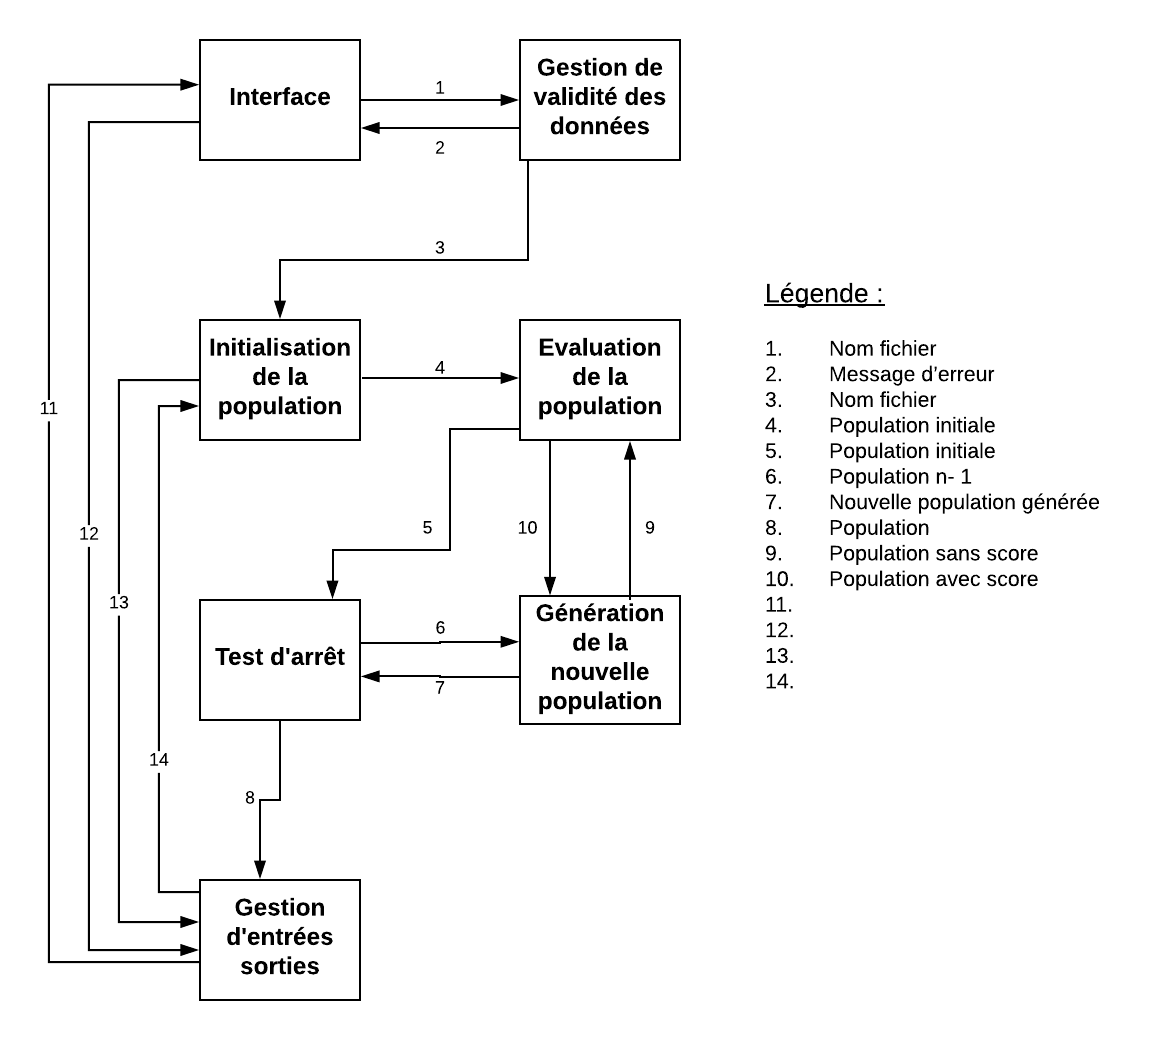
\includegraphics[width = 12cm,height = 10cm]{OrganigrammeV4.png}}
		
		Les données initiales sont : 	taux de mutation, 
										identifiant plus tableau pour le test, 
										fonction fitness, 
										nombre de génération, 
										score à atteindre sur la fonction, 
										taille individu, 
										critère d’évaluation, 
										nombre de critères, 
										alphabet, 
										taille population, probabilité de crossover, 
										nom de fichier.\\
		\\
		\underline{Interface :}
			\begin{itemize}
			\item Affichage des différents champs de saisie puis des résultats
			\item Réception des valeurs (Données initiales)
				\begin{itemize}
				\item par fichier
				\item par saisie des champs de l'interface
				\end{itemize}
			\item Option d’arrêt pendant l'exécution de l’AG : on peut arrêter le programme à tout moment et récupérer les résultats jusqu’à l’arrêt\\
			\end{itemize}
		
		\underline{Gestion de la validité des données : }
		\begin{itemize}
			\item Test des valeurs reçues
			\item Enregistrement des valeurs dans un fichier\\
		\end{itemize}
		
		\underline{Module d'initialisation : }
		\begin{itemize}
			\item Transformation de valeurs en paramètres
			\item Creation de la population initiale
			\item Lecture du fichier des données\\
		\end{itemize}
	
		\underline{Evaluation de la population : }
		\begin{itemize}
			\item Evaluation de chaques individus et attribution d'un score
		\end{itemize}
		\begin{tabbing} 
		Algo\=rithme Evaluation : paramètre : une population\\
			\>Si l\=e nombre de critères == 1\\
			\>	\>Si l\='option d'évaluation du critère == '>'\\
			\>	\>	\>Tri de la population puis attribution du score en fontion du rang après le tri\\
			\>Sinon
			\>	\>Pour chaque individu de la population faire :\\
			\>	\>	\>Utilisation de la fonction fitness, le score correspond au résultat renvoyé
		\end{tabbing}
		Complexité dans le pire des cas : O(k*n²) (k : nombre de critères, n : taille de la population)\\
		
		\underline{Tests d'arrets : }
		\begin{itemize}
			\item Test de convergence de la fonction fitness
			\item Test du nombre de générations\\
		\end{itemize}

		\underline{Génération de la nouvelle population : }
		\begin{itemize}
			\item Selection par roulette
			\item Cross-over/mutation
			\item Création de la nouvelle population
			\item Génération de nombres aléatoires
		\end{itemize}
		\begin{tabbing} 
		Algo\=rithme Roulette : paramètre : les individus\\
			\>si l\=e nombre d’individus est pair\\
			\>	\>limite = population/2\\
			\>sinon\\
			\>	\>limite = population-1/2\\
			\>scoremax = $\sum score$\\
			\>Pour chaque individus on calcule sa valeur (en pourcentage) en fonction du scoremax\\
			\>Tant qu’on a pas assez d’individu sélectionné\\
			\>	\>Si l\=e poucentage du premier individu est supérieur à une valeur aléatoire\\
			\>	\>\>il est sélectionné\\
			\>	\>Pour chaque individu sauf le premier faire :\\
			\>	\>\>si (l\=e pourcentage de l'individu > à une valeur aléatoire\\ 
			\>	\>\>ET que le pourcentage de celui qui le précède est inférieur à cette valeur)\\
			\>	\>\>\>cet individu est sélectionné.\\
			\>On retourne les individus sélectionné
		\end{tabbing}

		\underline{Gestion d'entrées sorties : }
		\begin{itemize}
			\item Calcul des statistiques de l'éxécution : les données d'entrées et les résultats
			\item Ecriture des résultats dans latex
			\item Ecriture des résultats dans PostScript
			\item Ecriture des résultats dans Xfig
			\item Lecture d'un fichier d'entrée avec les données
			\item Ecriture des valeurs dans un fichier\\
		\end{itemize}
		
		Dans tous les modules il faut une fonctionnalité qui lit les valeurs nécessaires dans le fichier des données.
		
	\section{Autres aspects du projet}
		\subsection{Estimation des coûts du projet}
		%~ \begin{center}
			%~ \begin{longtable}{|>{\centering}m{3cm}|>{\centering\arraybackslash}m{7cm}|>{\centering}m{4cm}|>{\centering}m{4cm}|}
				%~ \hline Modules & Nombre de lignes & Temps & Affectation\\
				%~ \hline \multicolumn{1}{|c|}{\textbf{Modules}} & \multicolumn{1}{c|}{\textbf{Nombre de lignes}} & \multicolumn{1}{|c|}{\textbf{Temps}} &\multicolumn{1}{|c|}{\textbf{Affectation}}\\
				%~ \hline Interface & 250-300 & 5-6 heures & Rémi et Edouard\\
				%~ \hline Gestion de la validité des données & 50-60 & 1-2 heures & Maxime et Laureline\\
				%~ \hline 
				%~ \multirow{3}{0cm}{Initialisation du programme} & transformation des valeurs en paramètres : 30 & 2-3 heures & Edouard et Rémi\\
																%~ & création de la population initiale : 40 & &\\ 
																%~ & lecture du fichier de données : 40 & &\\ 
				%~ \hline Evaluation de la population & 25-30 & 1-2 heures & Lydia et Ben\\
				%~ \hline 
				%~ \multirow{2}{0cm}{Tests d'arrets} & par itération ou forcé : 20 & 2-3 heures  & Laureline et Maxime\\
													%~ & par convergence : ?? (~50) & &\\
				%~ \hline Generation de la nouvelle population & 40-50 & 2-3 heures & Ben et Lydia\\
				%~ \hline Gestion d'entrées sorties & ~200 & 4-5 heures & tout le monde\\
				%~ \hline \textbf{Coût Total} & \textbf{XXX} & & \\
				%~ \hline 	
				%~ \end{longtable}\vspace{1em}
			%~ \end{center}
			
			
			
			\begin{center}\begin{longtable}{|>{\centering}m{3cm}|>{\centering}m{5cm}|>{\centering}m{3cm}|>{\centering\arraybackslash}m{3cm}|}			
				\hline \multicolumn{1}{|c|}{\textbf{Module}} & \multicolumn{1}{c|}{\textbf{Nombre de lignes}} & \multicolumn{1}{c|}{\textbf{Temps}} & \multicolumn{1}{c|}{\textbf{Affectation}} \\
				\hline 	Interface 								& 250-300 	& 5-6 heures 	& Rémi et Edouard		\\
				\hline 	Gestion de la validité des données 		& 50-60 	& 1-2 heures 	& Maxime et Laureline	\\
				\hline 	
				\multirow{3}{2cm}{Initialisation du programme}	& transformation des valeurs en paramètres : 30 & 2-3 heures & Edouard et Rémi\\
																& création de la population initiale : 40 & &\\ 
																& lecture du fichier de données : 40 & &\\
				\hline 	Evaluation de la population 			& 25-30 	& 1-2 heures	& Lydia et Ben			\\
				\hline  
				\multirow{2}{2cm}{Tests d'arrets} & par itération ou forcé : 20 & 2-3 heures  & Laureline et Maxime\\
												 & par convergence : ?? (~50) & &\\
				\hline 	Generation de la nouvelle population 	& 40-50 	& 2-3 heures	& Ben et Lydia			\\
				\hline 	Gestion d'entrées sorties 				& ~200 		& 4-5 heures	& tout le monde			\\
				\hline \textbf{Coût Total} & \textbf{565} & \textbf{environ 10000h} & \\
				\hline 	
				\end{longtable}\vspace{1em}\end{center}
				
		\subsection{Manuel utilisateur et formations}
		Un manuel d'utilisation sera fourni pour conseiller à l’utilisateur les données les plus performantes pour avoir des solutions plus efficaces.
	
	\section*{Conclusion}
		Pour résoudre les exigences du client, nous avons élaboré un cahier des charges qui décrit les différents dispositifs nécessaire pour conceptualiser un algorithme génétique générique. Dans ce cahier des charges, nous proposons une solution qui permettra au client de simuler des problèmes variés, tels que des problèmes génétiques, mathématiques, d’optimisation, etc., dont les solutions sont approchées et obtenir les résultats pour chaque générations. 
	Ce sujet nous intéresse tout particulièrement. De plus, l’écriture d’un cahier des charges est un travail inédit pour nous, il nous a permit de travailler en groupe de six personne pour la première fois, cela nous a appris à développer une organisation particulière.
	\newline
	Le langage qui nous semble le plus adapté est le C++. Nous choisissons un langage hybride. D’une part, nous aurons besoin d’un langage objet pour implémenter les individus. En effet, un individu sera un objet caractérisé par plusieurs champs. Les individus formeront une population qui sera elle aussi un objet. 
	D’autres part, nous aurons besoin d’un langage procédural afin d’effectuer des calculs sur les individus. Le C++ nous semble également avantageux dans l’utilisation d’un parser (utilisé avec la fonction fitness).

	\section*{Bibliographie}
	\begin{itemize}
		\item Présentation des algorithmes génétiques et de leurs applications en économie : 
		\newline
		http://deptinfo.unice.fr/twiki/pub/Minfo04/IaDecision0405/Prsentationdesalgorithmesgntiquesetdeleursapplicationsenconomie\_P.pdf

		\item La page wikipedia sur l'algorithme génétique : 
		\newline
		https://fr.wikipedia.org/wiki/Algorithme\_g%C3%A9n%C3%A9tique

		\item Tutoriel Python sur les algorithmes génétiques :
		\newline
		https://skyduino.wordpress.com/2015/07/16/tutorielpython-les-algorithmes-genetiques-garantis-sans-ogm/

		\item Etude sur les algorithmes génétiques :
		\newline
		http://souqueta.free.fr/Project/files/TE\_AG.pdf
		
		\item Exemple d'utilisation sur un jeu vidéo :
		\newline
		https://www.youtube.com/watch?v=9tCySY6TLk8

		\item Vidéos d'explications de l'algorthme génétique : 
		\newline
		https://www.youtube.com/watch?v=VOIPosVDkEE
		https://www.youtube.com/watch?v=bLdrDnZfpPo
		https://youtu.be/mAybMmf0veY

		\item L'application des algorithmes génétique dans la science des données :
		\newline
		https://www.analyticsvidhya.com/blog/2017/07/introduction-to-genetic-algorithm/ 


		\item Explications de l’aglorithme générique :
		\newline
		http://khayyam.developpez.com/articles/algo/genetic/
		http://informatique.coursgratuits.net/methodes-numeriques/algorithmes-genetiques.php

		\item Etude sur l'inertage de feu :
		\newline
		http://www.ligeron.com/telecharger.php?id=11

		\item Comparaison de l'algorithme génétique et du réseau de neuronnes :
		\newline
		https://stackoverflow.com/questions/1402370/when-to-use-genetic-algorithms-vs-when-to-use-neural-networks
	\end{itemize}
	

\end{document}
